\documentclass{article}
\usepackage[english]{babel}
\usepackage[utf8x]{inputenc}
\usepackage[fleqn]{amsmath}
\usepackage{amssymb}
\usepackage{graphicx}
\usepackage[colorinlistoftodos]{todonotes}
\usepackage{geometry}
\geometry{hmargin=2.0cm,vmargin=1.5cm}
\usepackage{wrapfig}	% Figures avec du texte autour
\usepackage{lipsum}

\title{Anisotropic equivalent fluid identification}
\author{Arthur TERROIR}
\date{\today}

\begin{document}
\maketitle

%%%%%%%%%%%%%%%%%%%%%%%%%%%%%%%%%%%%%%%%%%%%%%%%%%%%%%%%%%%%%%%%%%%%%%
\section{Introduction}


%%%%%%%%%%%%%%%%%%%%%%%%%%%%%%%%%%%%%%%%%%%%%%%%%%%%%%%%%%%%%%%%%%%%%%
\section{Description of the configuration}
    The material studied is a layer of equivalent fluid, with anisotropic complex density as follow : 
    \begin{align}
        \Bar{\Bar{\rho}}=\begin{pmatrix}
    					\rho_{1} & \rho_{12} & \rho_{13} \\
                        \rho_{12} & \rho_{2} & \rho_{23} \\
                        \rho_{13} & \rho_{23} & \rho_{3}\end{pmatrix}\label{Density_tensor}.
    \end{align}
    The propagation problem is described on the figure (\ref{Schema_PB}), the medium is excited with a acoustic harmonic plane wave on $x_3=L$. The fluid layer is supposed to be infinite along the plan $x_1x_2$ and with a debt L along $x_3$. The incident wave is oriented with two angle , elevation $\theta$ and azimuthal $\phi$, the three projected wave number are :   
   \begin{align*}
    &k_1=-k_0 sin(\theta) cos(\phi), \\
    &k_2=-k_0 sin(\theta) sin(\phi), \\
    &k_3= -k_0 cos(\theta),
    \end{align*}
    where $k^{(0)}$ is the incident wave number at the radial frequency $\omega$. 
    
    \begin{figure}[ht]
        \centering
        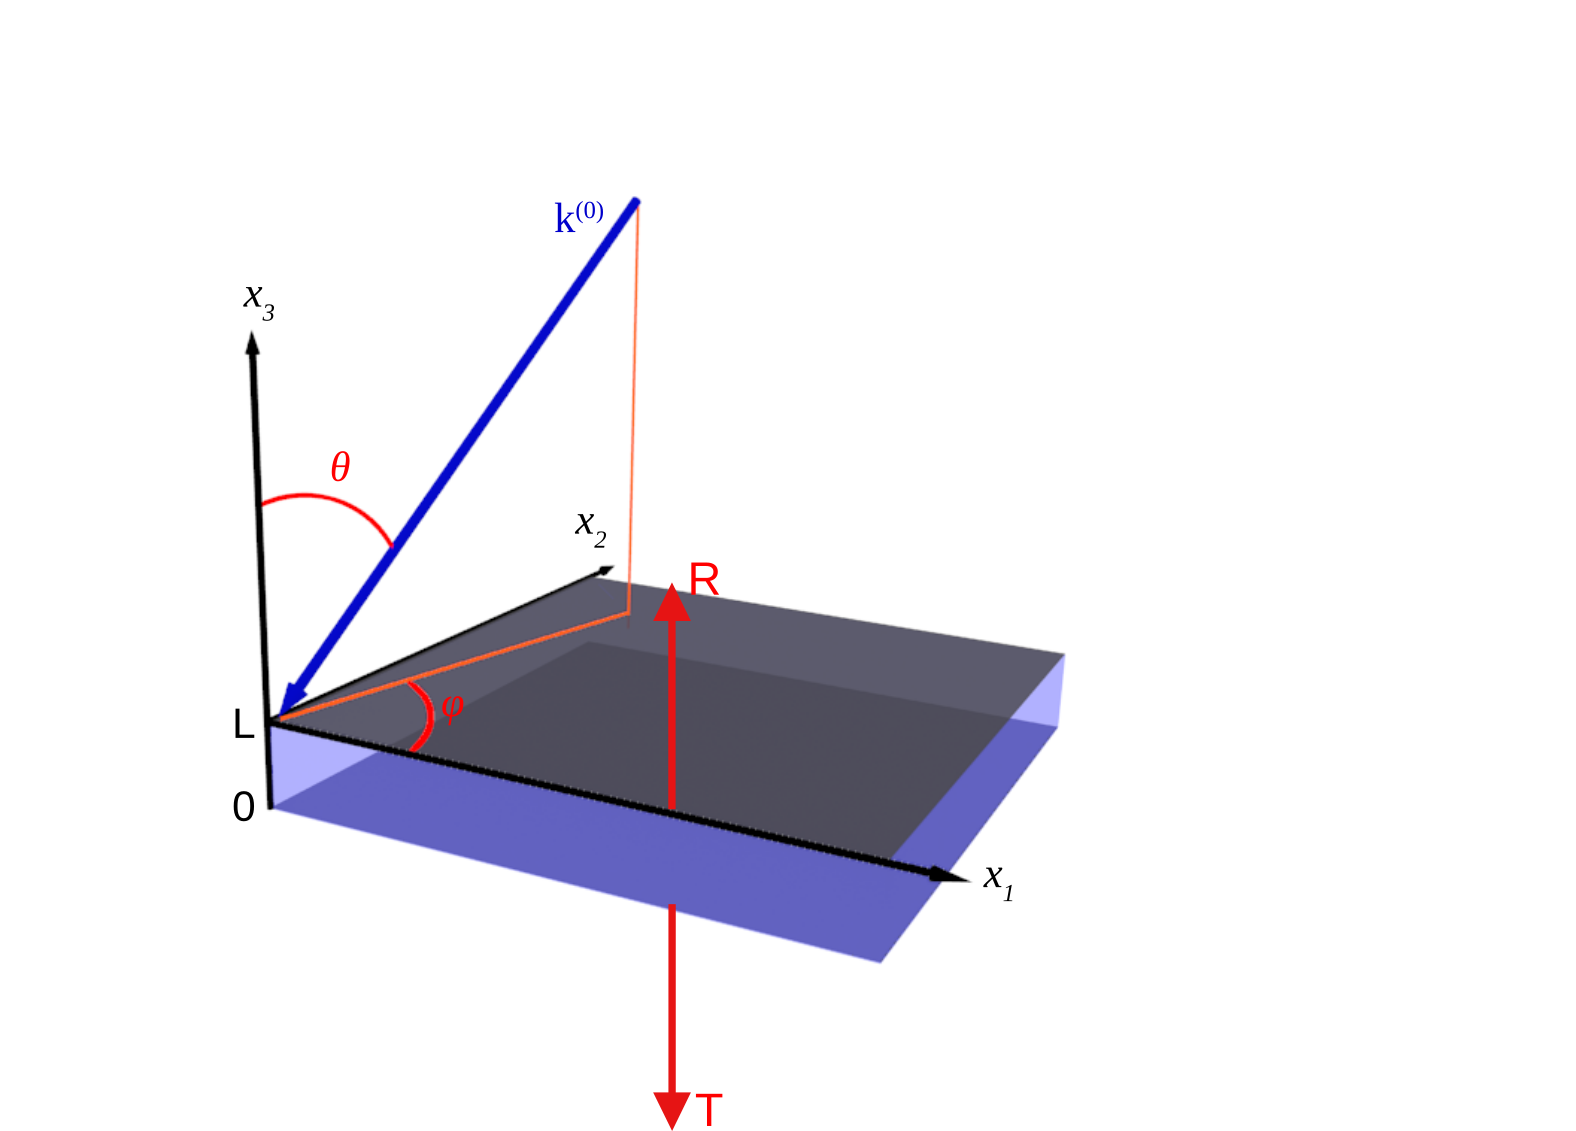
\includegraphics[scale=0.6]{Fig3D.png}
        \caption{azerty}
        \label{Schema_PB}
    \end{figure}
    
    Considering the propagation problem, the boundary condition are defined using the reflection and transmission coefficient, the incident and reflected wave are observed on the interface at $x_3=L$ and the transmitted wave at $x_3=0$, the boundary condition can be write as :
     \begin{align}
    &\bar{S}_{(L)}=\begin{pmatrix}
    	p \\ v_3
    \end{pmatrix}_{(L)}=\begin{pmatrix}
    					    1+R \\ -\frac{k_3}{\rho \omega}(1-R),
    					\end{pmatrix},\label{BC_L} \\
  	&\bar{S}_{(0)}=\begin{pmatrix}
    	p \\ v_3
    \end{pmatrix}_{(0)}=\begin{pmatrix}
    						Te^{ik_3L} \\ -\frac{k_3}{\rho \omega}Te^{ik_3L}
    					\end{pmatrix},\label{BC_0}
    \end{align}                         
    with $\bar{S}$ the state vector (pressure and particle velocity) of the wave propagating, and R and T, the reflection coefficient at $x_3=L$ and the transmission coefficient at $x_3=0$.  
    
%%%%%%%%%%%%%%%%%%%%%%%%%%%%%%%%%%%%%%%%%%%%%%%%%%%%%%%%%%%%%%%%%%%%%%
\section{Parameters identification}
\subsection{Transfer Matrix}
    To achieve the parameters identification, the transfer matrix of the fluid should be known to describe the propagation of the wave between the two interface. It's here proposed to derive the transfer matrix using the following Euler's equation :
    \begin{align}
        &\rho \frac{\partial}{\partial t}v=-\nabla p, \\
	    &\frac{\partial}{\partial t}p=-K\nabla v,
    \end{align}
    The solutions are supposed to be harmonic plane wave, of angular frequency $\omega$, write as, with the time convention $e^{-i\omega t}$ :
    \begin{align}
        \xi=\tilde{\xi}e^{i(k_1 x_1+k_2 x_2)}e^{-i\omega t}
    \end{align}
    Introducing the density matrix $\bar{\bar{\rho}}$ (eq. (\ref{Density_tensor})), the Euler expressions become :
    \begin{align}
	    &ik_ip=\sum_{j=1}^{3} i \omega \rho_{ij} v_j,\ i=1,2\label{Euler1}\\
	    &\frac{\partial}{\partial x_3}p=\sum_{j=1}^{3} i \omega \rho_{3j} v_j\label{Euler2}\\
        &i\omega p= iK(k_1v_1+k_2v_2+\frac{\partial}{\partial x_3}v_3).\label{Euler3}
    \end{align}
    Using the expressions (\ref{Euler1}), the particle velocity $v_1$ and $v_2$ can be express a function of the state vector $\bar{S}$, and and introducing this function in the expressions (\ref{Euler2}) and (\ref{Euler3}), the propagation matrix $\bar{\bar{A}}$ can be derive as :
    \begin{align}
        &\frac{\partial}{\partial x_3}\bar{S} = \bar{\bar{A}} \bar{S},\label{Equa_diff}
        \intertext{with :}
        &\bar{\bar{A}}=\begin{pmatrix}
    				A_{11} & A_{12} \\ A_{21} & A{22}
    			\end{pmatrix}\label{Matrice_complete},\\ 
         &A_{11}=A_{22}=i[\frac{\rho_{22}\rho_{13}-\rho_{12}\rho_{23}}{\rho_{11}\rho_{22}-\rho_{12}^2}k_1+\frac{\rho_{11}\rho_{23}-\rho_{12}\rho_{13}}{\rho_{11}\rho_{22}-\rho_{12}^2}k_2], \\
     &A_{12}=i\omega \rho_{33}[1-\frac{\rho_{13}}{\rho_{11}\rho_{22}-\rho_{12}^2}(\frac{k_1^{(i)}}{k_3^{(i)}})^2(\rho_{22}-\rho_{12}(\frac{k_2^{(i)}}{k_1^{(i)}})^2)-\frac{\rho_{23}}{\rho_{11}\rho_{22}-\rho_{12}^2}(\frac{k_2^{(i)}}{k_3^{(i)}})^2(\rho_{11}-\rho_{12}(\frac{k_1^{(i)}}{k_2^{(i)}})^2)], \\
     &A_{21}=\frac{i\omega}{K}[1-\frac{\rho_{33}}{\rho_{11}\rho_{22}-\rho_{12}^2}(\frac{k_1}{k_3^{(i)}})^2(\rho_{22}-\rho_{12}\frac{k_2}{k_1})-\frac{\rho_{33}}{\rho_{11}\rho_{22}-\rho_{12}^2}(\frac{k_2}{k_3^{(i)}})^2(\rho_{11}-\rho_{12}\frac{k_1}{k_2})],
    \end{align}
    where $k_m^{(i)}$ is a effective wave number along the direction m, independent of the frequency, such as $k_m^{(i)}=\frac{\omega}{\sqrt{\frac{K}{\rho_{m3}}}}$.
    
    The propagation matrix can be express with new parameter, consider as the effective parameters of the anisotropic fluid. Using the four terms of the equation (\ref{Matrice_complete}), 4 parameters can be identified, the effective bulk modulus $\tilde{K}$, the effective density $\tilde{\rho_3}$ along the propagation direction and two phase-shift terms $q_1$ and $q_2$ link to the non-planar anisotropy.
    
    \begin{align}
     &\tilde{K}=\frac{K}{[1-\frac{\rho_{33}}{\rho_{11}\rho_{22}-\rho_{12}^2}(\frac{k_1}{k_3^{(i)}})^2(\rho_{22}-\rho_{12}\frac{k_2}{k_1})-\frac{\rho_{33}}{\rho_{11}\rho_{22}-\rho_{12}^2}(\frac{k_2}{k_3^{(i)}})^2(\rho_{11}-\rho_{12}\frac{k_1}{k_2})]}\label{Ktild},\\
     &\tilde{\rho_3}=\rho_{33}[1-\frac{\rho_{13}}{\rho_{11}\rho_{22}-\rho_{12}^2}(\frac{k_1^{(i)}}{k_3^{(i)}})^2(\rho_{22}-\rho_{12}(\frac{k_2^{(i)}}{k_1^{(i)}})^2)-\frac{\rho_{23}}{\rho_{11}\rho_{22}-\rho_{12}^2}(\frac{k_2^{(i)}}{k_3^{(i)}})^2(\rho_{11}-\rho_{12}(\frac{k_1^{(i)}}{k_2^{(i)}})^2)]\label{rho3tild}, \\
	&q_{1}=\frac{\rho_{22}\rho_{13}-\rho_{12}\rho_{23}}{\rho_{11}\rho_{22}-\rho_{12}^2}k_1\label{q1},\\
    &q_{2}= \frac{\rho_{11}\rho_{23}-\rho_{12}\rho_{13}}{\rho_{11}\rho_{22}-\rho_{12}^2}k_2\label{q2}.
          \end{align}
          
    The transfer matrix can be obtain knowing the propagation matrix, resolving the equation (\ref{Equa_diff}), so :
    \begin{align}
    \bar{S}_{(l)}=e^{\bar{\bar{A}}L}\bar{S}_{(0)}.\label{PB}
    \end{align}
    In this case, $e^{\bar{\bar{A}}L}$ is the transfer matrix allowing the characterization of the propagation between the two interfaces of the medium.
    To know the analytic expression of the transfer matrix $Tr$, the propagation matrix $\bar{\bar{A}}$ should be diagonalize, so the matrix exponential can be derive.
    With the diagonalization, the propagation matrix can be express as :
     \begin{align}
    \bar{\bar{A}}=\bar{\bar{U}} \begin{pmatrix}
    								-ik_{33}+i\tilde{q} & 0 \\ 0 & ik_{33}+i\tilde{q} 
    							\end{pmatrix} \bar{\bar{U^{-1}}},
    \end{align}
    where U is the eigen vector $\bar{\bar{U}}=\frac{1}{\sqrt{2}}\begin{pmatrix} Z_3 & Z_3 \\ -1 & 1 \end{pmatrix}$, $k_{33}$ the effective wave number along $x_3$ as $k_{33}=\frac{\omega}{c_{33}}=\frac{\omega}{\frac{\tilde{K}}{\tilde{\rho_3}}}$, $\tilde{c_{33}}$ the effective celerity, $Z_3$ the effective impedance as $Z_3=\tilde{\rho_3c_{33}}$, and $\tilde{q}$ is the global phase-shift terms $\tilde{q_1+q_2}$.
    
    Then it come the following transfer matrix $Tr$ :
        \begin{align}
    Tr=\bar{\bar{U}}\begin{pmatrix}
    e^{-ik_{33}L} & 0 \\ 0 & e^{-ik_{33}L} 
    \end{pmatrix} e^{i\tilde{q}L}\bar{\bar{U^{-1}}}\label{Transfer_Matrix}
    \end{align}
    
    Notice that using using the boundary condition (\ref{BC_L}) and (\ref{BC_0}), and introducing the expression (\ref{Transfer_Matrix}) in the equation  (\ref{PB}), it can be show that the reflection and transmission coefficients can be write as :
        \begin{align}
    &T=\frac{e^{-i\tilde{q}L}}{cos(k_{33}L)-\frac{i}{2}(\frac{Z}{Z_3}+\frac{Z_3}{Z})sin(k_{33}L)}\label{Transmission},\\ 
    &R=\frac{i}{2} \frac{(\frac{Z}{Z_3}-\frac{Z_3}{Z})sin(k_{33}L)}{cos(k_{33}L)-\frac{i}{2}(\frac{Z_3}{Z}+\frac{Z}{Z_3})sin(k_{33}L)}\label{Reflexion}. 
      \end{align}

\subsection{Identification}
    The propagation between the two interfaces of the layer is now known with the transfer matrix (\ref{Transfer_Matrix}), an identification can be develop based on a inverse method. If the reflection and transmission are supposed to be the known parameters of the problem, the parameter to determine are the complex densities and the bulk modulus. Notice that the length of the layer L is supposed to be previously determine.
    
    To achieve the inverse propagation method, it's proposed here to take information from 6 angle of incidence, at first a view, using 6 angle of incidence for R and T induce 12 information to determine 7 parameters (6 density and the bulk modulus), so the method seems oversized. The excess of information come from the redundant information of the bulk modulus, in fact for all the angle of incidence, the information of the bulk modulus is present. 
    
\subsubsection*{F(R,T,$\tilde{q}$)}
    The first step of the inverse method is to obtain an information about the propagation between the 2 interface of the layer using R and T, so it's proposed here to rewrite the propagation equation so parameters containing the propagation information can be express. 
    
    Introducing the analytic expression of the transfer matrix $Tr$ (\ref{Transfer_Matrix}) in the differential equation (\ref{PB}), the propagation equation become :
    \begin{align}
    \bar{\bar{U^{-1}}} \bar{S}_{(L)}= \begin{pmatrix}
                                   			e^{-ik_{33}L} & 0 \\ 0 & e^{ik_{33}L}
                                            \end{pmatrix}e^{i\tilde{q}} \bar{\bar{U^{-1}}} \bar{S}_{(0)}, 
   \end{align} 
    Developing, it come 2 expressions  :
    \begin{align}
	&e^{i k_{33}L}=\frac{(1+R)-\frac{Z_3}{Z}(1-R)}{(1-\frac{Z_3}{Z})T}e^{-i\tilde{q}L},\label{k_33_tmp1}\\
    &e^{-i k_{33}L}=\frac{(1+R)+\frac{Z_3}{Z}(1-R)}{(1+\frac{Z_3}{Z})T}e^{-i\tilde{q}L}.\label{k_33_tmp2}
    \end{align} 

    At this point, there's 2 possibility of using the new equation of propagation, the first and the one that will be use for the resolution is to make the product of the (\ref{k_33_tmp1}) and (\ref{k_33_tmp2}) to cancel the $k_{33}$ terms and obtain the effective impedance $Z_3$ as a function of R,T and the characteristic impedance $Z$. Note that $Z$ is defined by the medium of the incident wave as $Z=\frac{\rho \omega}{k_3}$.
    The impedance $Z_3$ can express as, with the product (\ref{k_33_tmp1}).(\ref{k_33_tmp2}) :
    \begin{align}
    Z_3^2=\frac{T^2e^{2i\tilde{q}L}-(1+R)^2}{T^2e^{2i\tilde{q}L}-(1-R)^2}Z^2\label{Z3}.
    \end{align}
    
    A function $F(R,T,\tilde{q})$ is defined, so it can be write :
    \begin{align}
        Z_3=F(R,T,\tilde{q}),\\
        F(R,T,\tilde{q})=\sqrt{\frac{T^2e^{2i\tilde{q}L}-(1+R)^2}{T^2e^{2i\tilde{q}L}-(1-R)^2}}1.
    \end{align}
    
    Another way of extracting the propagation information is to know the effective wave number $k_{33}$ using one of the two equation (\ref{k_33_tmp1}) and (\ref{k_33_tmp2}).
    In the current state of the problem, the phase-shift term $\tilde{q}$ is not known yet, so both of $k_{33}$ and $Z_3$ are unknown. It's know from the expression (\ref{q1}) and (\ref{q2}) that $\tilde{q}$ is null in normal incidence, then both of $k_{33}$ and $Z_3$ can be determined in this case. Reminding that $Z_3=\tilde{\rho_3}c_{33}=\sqrt{\tilde{\rho_3}\tilde{K}}$
    
    
\subsubsection*{$\tilde{q}$}
\subsubsection*{$\rho_1$, $\rho_2$, $\rho_{12}$}
\subsubsection*{Restes}

%%%%%%%%%%%%%%%%%%%%%%%%%%%%%%%%%%%%%%%%%%%%%%%%%%%%%%%%%%%%%%%%%%%%%%
\section{Results}
    
    \begin{figure}[ht]
        \centering
        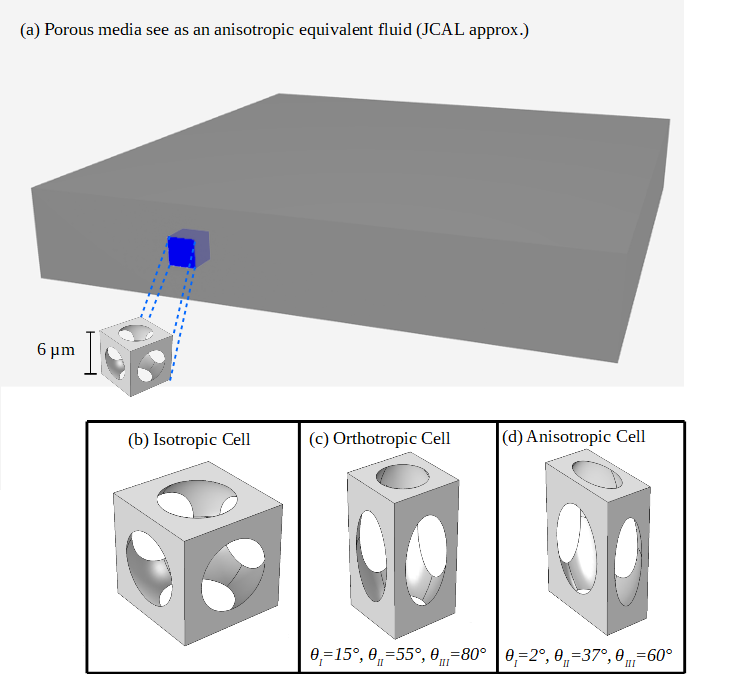
\includegraphics[scale=0.5]{Material_2.png}
        \caption{azerty}
        \label{Material}
    \end{figure}

    \begin{figure}[ht]
        \centering
        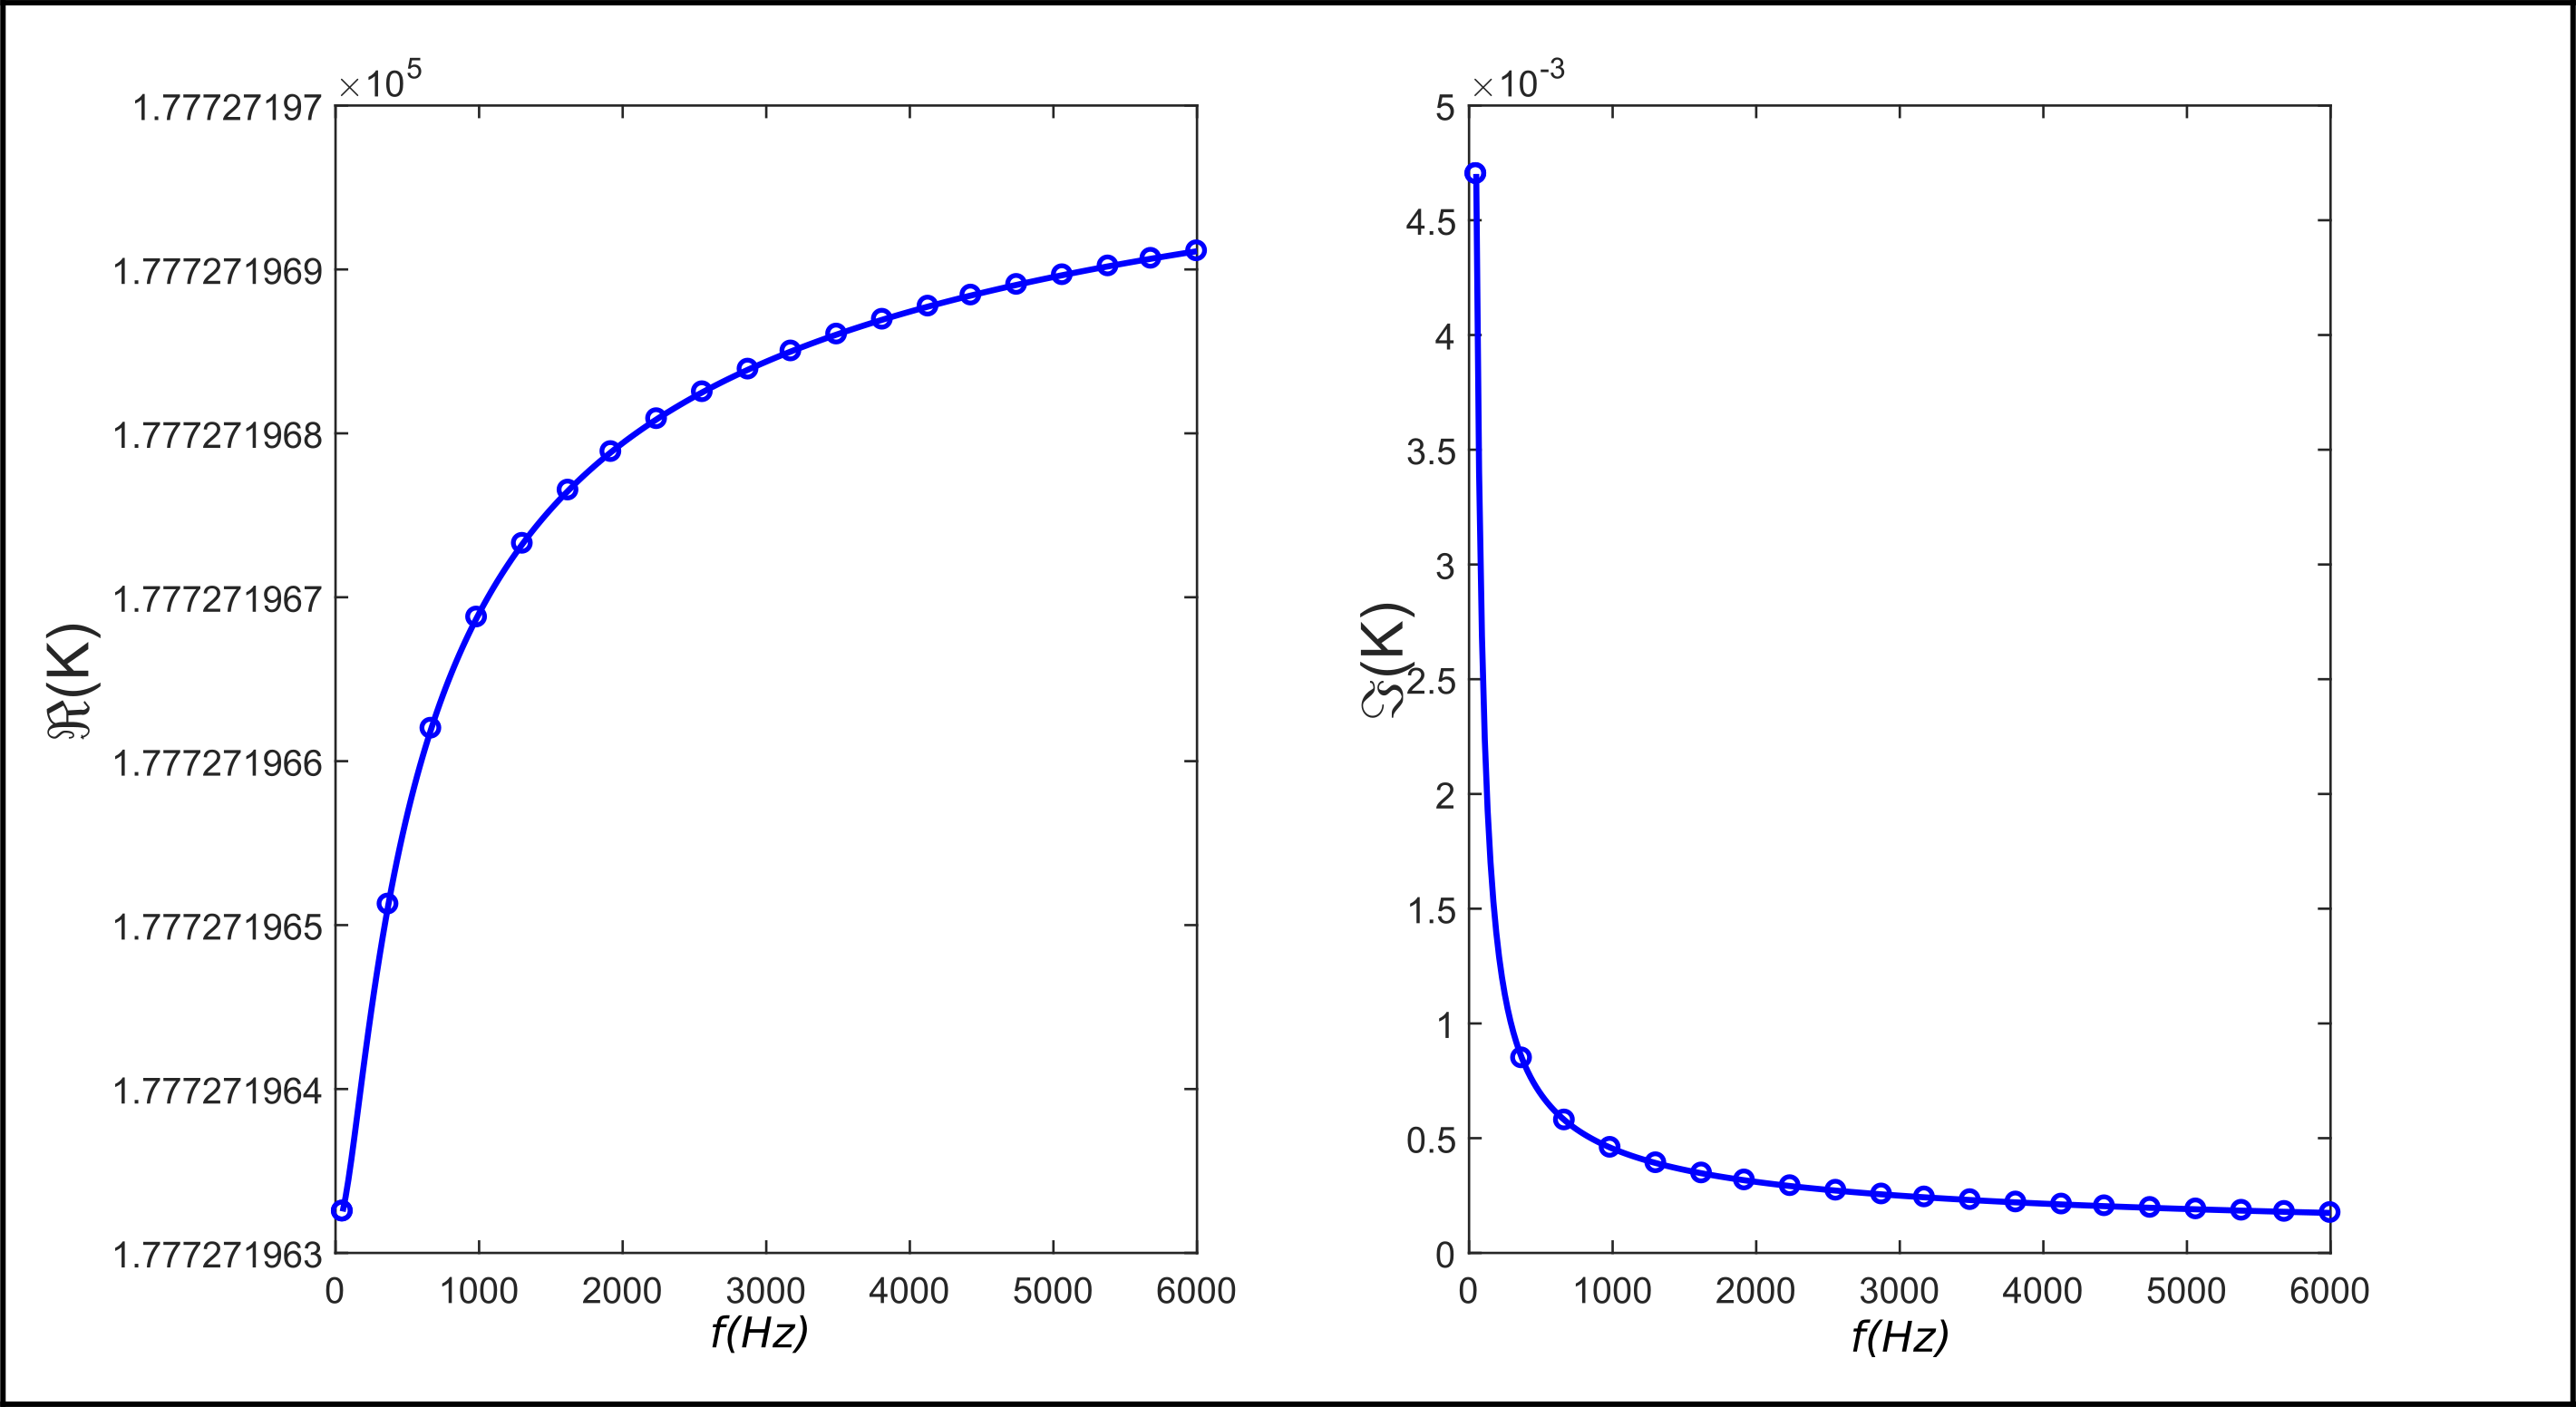
\includegraphics[scale=0.3]{Bulk.png}
        \caption{azerty}
        \label{Grph_K}
    \end{figure}

    \begin{figure}[ht]
        \centering
        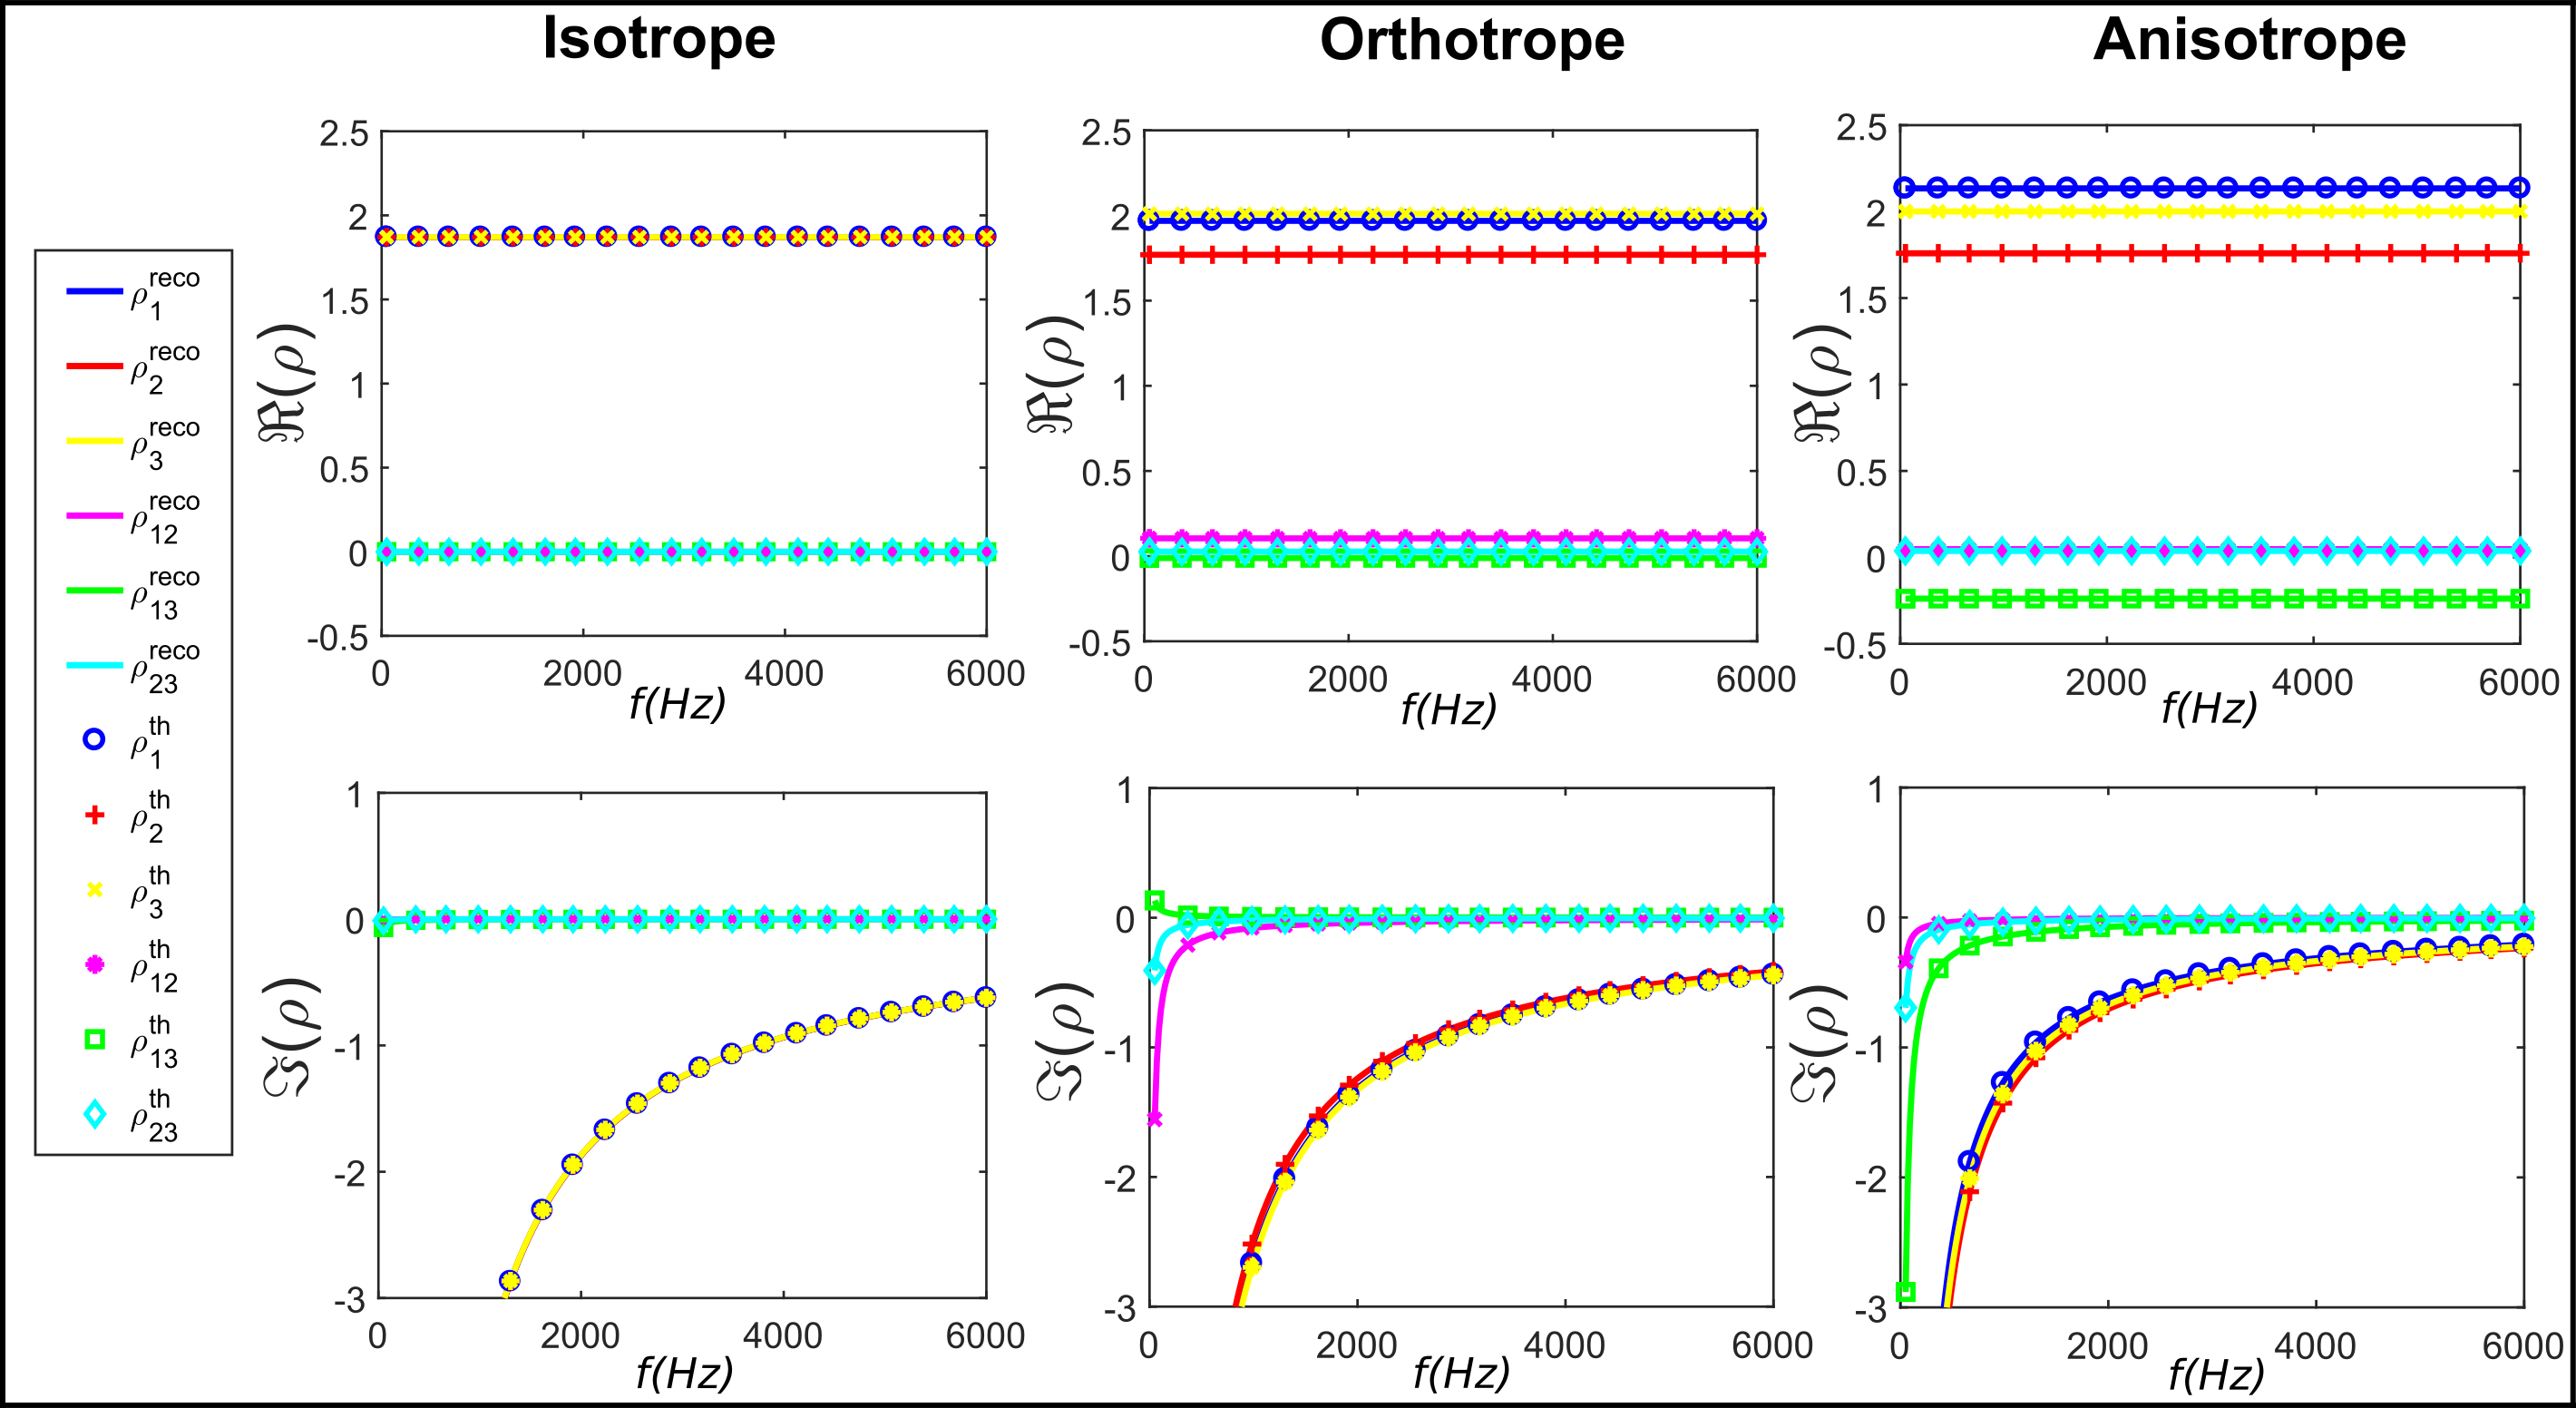
\includegraphics[scale=0.3]{Density_rot.png}
        \caption{azerty}
        \label{Grph_rho_rot}
    \end{figure}


    \begin{figure}[ht]
        \centering
        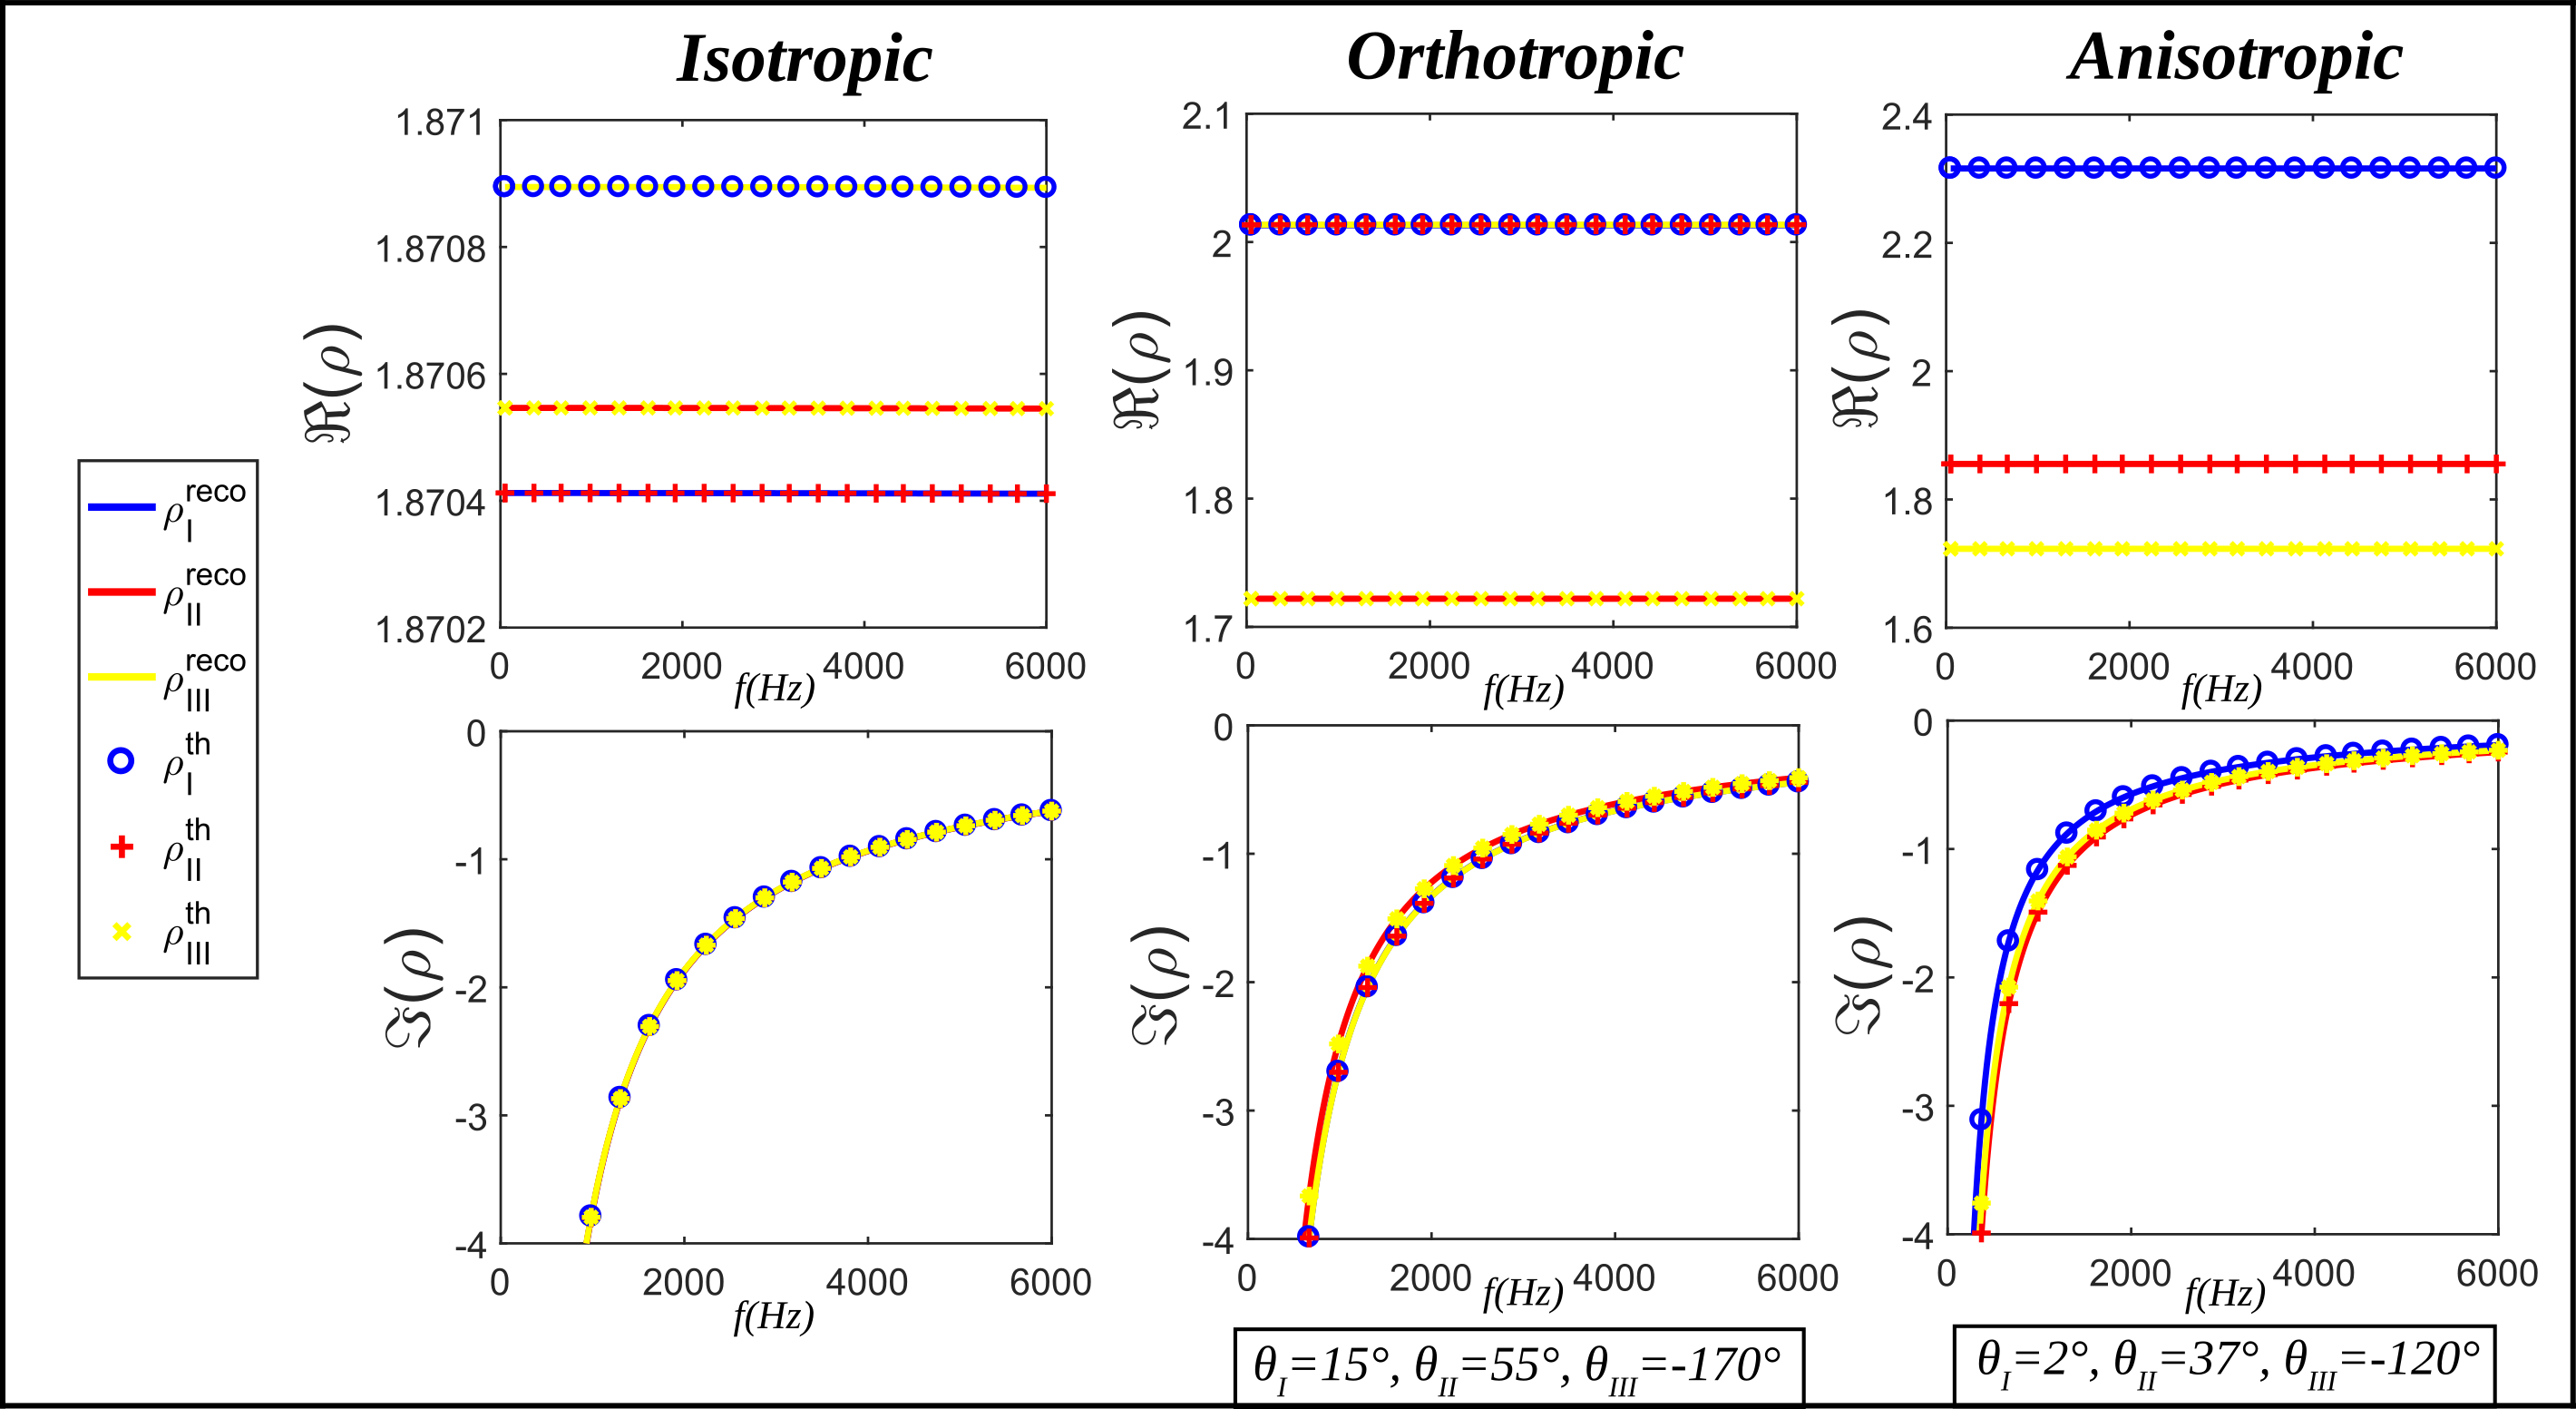
\includegraphics[scale=0.3]{Density_dir.png}
        \caption{azerty}
        \label{Grph_rho_dir}
    \end{figure}
%%%%%%%%%%%%%%%%%%%%%%%%%%%%%%%%%%%%%%%%%%%%%%%%%%%%%%%%%%%%%%%%%%%%%%
\section{Conclusion}


%%%%%%%%%%%%%%%%%%%%%%%%%%%%%%%%%%%%%%%%%%%%%%%%%%%%%%%%%%%%%%%%%%%%%%
\section{Annexe}
\end{document}
